\documentclass[10pt,conference,compsocconf]{IEEEtran}
\usepackage{amsmath,graphicx,booktabs}
\begin{document}
\title{NumPy Models for Survey-Based Heart Disease Classification}
\author{CS-433 Project 1: Reproducible Experimental Report}
\maketitle
\begin{abstract}
We implement six course estimators and study a reproducible NumPy pipeline for classifying self-reported heart disease. The supplied dataset contains 328,135 labeled observations and 321 features, with 8.83\% positive labels and 44.79\% missing feature values. A stratified training/tuning/holdout protocol separates model and threshold selection from final evaluation. Among four prespecified configurations, category-expanded logistic regression with L2 coefficient $10^{-4}$ achieves tuning F1 0.4277 and holdout F1 0.4199. Threshold selection has a substantially larger measured effect than category expansion. Refitting on all labeled data produces 109,379 test predictions. No competition score is claimed.
\end{abstract}

\section{Task and experimental protocol}
The course dataset contains BRFSS survey responses. The binary target indicates self-reported diagnosed coronary heart disease, myocardial infarction or angina, according to the project description. We map $-1,+1$ to $0,1$ during classification training and restore the original labels for submission. Each test identifier is preserved. This is retrospective classification of survey labels; a random survey split does not establish prediction of future events.

Class imbalance motivates reporting precision, recall and F1 alongside accuracy. Predicting every respondent negative already achieves 91.17\% holdout accuracy but zero F1. We therefore choose configurations by tuning F1 rather than accuracy. This is our local experimental objective, without assuming an unverified competition scoring rule.

Using NumPy's default random generator with seed 433, we independently shuffle the indices of each class and partition each at 60\% and 80\%. The resulting sets have 196,881 training, 65,627 tuning and 65,627 holdout rows. Within each set we shuffle again. All feature statistics use training data only. Each model's threshold maximizes tuning F1, and the configuration with highest tuning F1 is selected. Only after this decision do we evaluate the holdout set. We use a single stratified split, not cross-validation. The delivered split-index file fixes the exact allocation.

\section{Feature processing}
Missing entries are represented by NaN. Of 321 original columns, we exclude explicitly named survey collection and weighting fields: state, interview month/date/year, disposition, sequence and primary sampling identifiers, stratum, and survey weight/raking variables. The exact list appears in \texttt{pipeline.py}. We also discard columns with fewer than 20\% observed training entries or fewer than two distinct observed values. This rule reduces noise and avoids fitting mostly absent survey modules.

In the numeric representation, we impute each retained column with its training median, clip to its observed training 1st and 99th percentiles, and standardize using the mean and standard deviation of the clipped, imputed training column. The minimum scale is $10^{-6}$. A separate indicator records each retained column's original missingness. An intercept is added. This gives 373 design columns on the training partition.

The category representation treats a column as categorical if it has 2--20 distinct observed training values. We encode each observed level except the smallest and append a missing indicator. Other columns use the numeric procedure above. Unseen levels have the same zero category vector as the reference level. This heuristic gives 717 design columns. Survey codes for refusal or unknown responses are retained as levels for categorical columns; numeric codes are clipped rather than assigned undocumented meanings. Thus the method avoids assuming a clinical codebook that was not supplied, but may lose useful semantics.

\section{Implemented estimators and training}
All six required estimators return the last weights and their corresponding unpenalized loss. Least-squares objectives use
\[
L_{\rm MSE}(w)=\frac{1}{2N}\|y-Xw\|_2^2.
\]
Full gradient descent updates with $X^T(Xw-y)/N$; stochastic gradient descent samples exactly one observation uniformly per iteration. Least squares solves the normal equations, with a pseudoinverse fallback for a singular Gram matrix. It does not call \texttt{numpy.linalg.lstsq}. Ridge adds $2N\lambda I$ to the Gram matrix, corresponding to $L_{\rm MSE}+\lambda\|w\|_2^2$.

Logistic regression uses mean binary cross-entropy, computed with \texttt{logaddexp} for numerical stability. Its gradient is $X^T(\sigma(Xw)-y)/N$. The regularized required function adds $2\lambda w$ to the gradient but excludes the penalty from its returned loss. Initial weights are copied to avoid mutating caller inputs. Zero iterations evaluate the supplied weights.

\clearpage
\section{Comparisons and results}
Our additional logistic optimizer uses minibatch Adam for efficiency, with unweighted cross-entropy and L2 regularization excluding the intercept. We use 16 epochs, batch size 4,096, $\beta_1=0.9$, $\beta_2=0.999$, $\epsilon=10^{-8}$ and learning rate $0.01/(1+e/10)$ at zero-based epoch $e$. Non-intercept weights start at zero; the intercept starts at the training prevalence log-odds. The shuffle seed is 433. These settings remain fixed across logistic experiments.

We compare numeric ridge at $\lambda=10^{-3}$, numeric logistic at $10^{-4}$, and categorical logistic at $10^{-4}$ and $10^{-3}$. For each fit, we sort tuning scores, accumulate true positives, and evaluate F1 only at distinct-score boundaries; this handles ties exactly. We select the score threshold yielding maximum F1, with larger thresholds winning an exact tie. The resulting thresholds are 0.20956, 0.20257, 0.18887 and 0.20956, respectively. Ridge scores are unconstrained regression outputs, rather than probabilities.

\begin{table}[h]
\centering
\caption{Measured performance. Thresholds use tuning labels only. All values are proportions; categorical logistic with $10^{-4}$ is selected by tuning F1.}
\small
\setlength{\tabcolsep}{3.5pt}
\begin{tabular}{lrrrr}
\toprule
Model & $\lambda$ & Tune F1 & Test F1 & Test acc.\\
\midrule
Always negative & -- & -- & 0.0000 & 0.9117\\
Numeric ridge & $10^{-3}$ & 0.4176 & 0.4113 & 0.8581\\
Numeric logistic & $10^{-4}$ & 0.4255 & 0.4154 & 0.8636\\
Category logistic & $10^{-4}$ & 0.4277 & 0.4199 & 0.8658\\
Category logistic & $10^{-3}$ & 0.4248 & 0.4181 & 0.8767\\
\bottomrule
\end{tabular}
\end{table}

\begin{figure}[h]
\centering
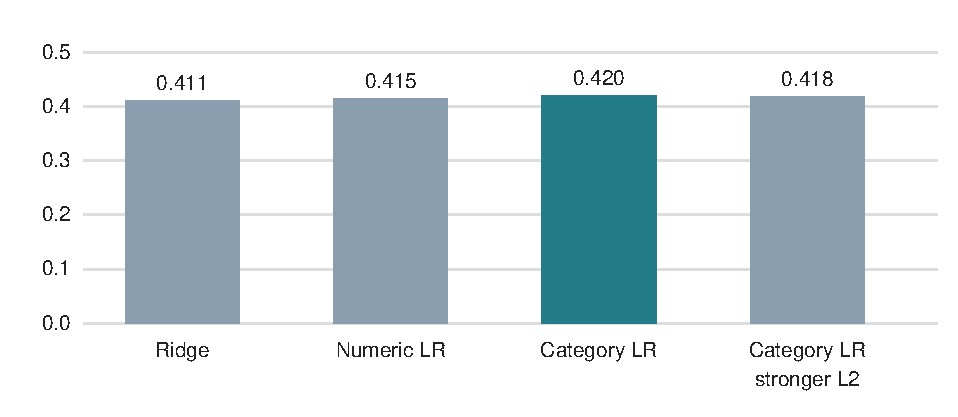
\includegraphics[width=\columnwidth]{comparison.pdf}
\caption{F1 on the untouched labeled holdout partition. ``Test'' in Table I refers to this partition, not the competition test set. These modest differences come from one split and are not significance claims.}
\end{figure}

Replacing numeric ridge with numeric logistic increases holdout F1 by 0.0041. Category expansion then adds 0.0045, while stronger regularization reduces the selected category model's holdout F1 by 0.0019. These are descriptive comparisons using frozen configurations; no hyperparameters were adjusted after observing the holdout results. The tuning-to-holdout gap for the selected model is 0.0077.

\subsection{Decision-threshold ablation}
For the selected categorical model, threshold 0.5 yields holdout F1 0.2339, precision 0.5538, recall 0.1482 and accuracy 0.9142. The tuning-selected threshold 0.18887 gives F1 0.4199, precision 0.3397, recall 0.5500 and accuracy 0.8658. Thus threshold choice raises F1 by 0.1861 and captures many more positives, at the expense of false alarms. This effect is considerably larger than the category-encoding gain. It illustrates why a single accuracy number is insufficient for this imbalanced task.

At the selected threshold the confusion counts are 3,187 true positives, 6,196 false positives, 2,608 false negatives and 53,636 true negatives. About 45\% of positive labels remain missed, and only about one third of positive predictions are correct. These errors limit practical interpretation despite the improvement over the majority baseline.

\section{Reproducibility and limitations}
After freezing the configuration and threshold, we refit preprocessing and logistic weights on all 328,135 labeled rows with the same training settings. We retain the tuning-selected threshold and generate 109,379 predictions. The reported holdout metrics apply to the model fitted on the 60\% training partition; they are not measured performance of the final all-data fit. Refitting can change the score distribution, so threshold transfer remains an assumption. Neither competition labels nor online scores were available.

The submission includes \texttt{run.py}, all six required estimators, the fitted preprocessor and weights, split indices, measured JSON results and the prediction CSV. Training and inference require only NumPy and standard Python libraries; ReportLab is used only to draw this figure. The supplied helper writes the required Id/Prediction columns and $-1,+1$ labels. The inference option loads the fitted model; full execution repeats model comparison and refitting. Fixed seeds ensure repeatable sampling, while different numerical libraries may introduce small arithmetic differences.

The small search and one split do not establish that this is the best possible model. Categorical detection is heuristic, numeric sentinel values are imperfectly handled, and no interactions are engineered. Several health and rehabilitation responses can follow diagnosis; without temporal definitions, their availability may inflate apparent prospective usefulness. A deployment-oriented study would audit those features, distinguish prior diagnosis from future disease, evaluate calibration and subgroup errors, and use repeated or external validation. Our claims are limited to the supplied survey classification experiment.
\end{document}
